\documentclass{scrartcl}

\usepackage[top=3cm, bottom=4cm, left=2cm, right=2cm]{geometry}
\usepackage[ngerman]{babel}
\usepackage{hyperref}
\usepackage{tcolorbox}
\usepackage{csquotes}
\usepackage{fontawesome}

% TODO:
\definecolor{hintboxcolor}{rgb}{0.5,0.5,0.5}
\definecolor{myurlcolor}{rgb}{0.3,0.3,0.6}

\hypersetup{
	colorlinks,
	urlcolor=myurlcolor
}

\title{\vspace{-2cm}Anleitung für die Abgabe der Programmieraufgaben über GitLab}
% TODO:
%\subtitle{}
%\author{}
%\date{}

\begin{document}
	\maketitle
	
	\begin{enumerate}
		\item Öffnen Sie das GitLab und loggen Sie sich mit Ihren Uni-Account-Daten ein:
		
		\vfill
		
		\url{<YOUR_GITLAB_URL>} % TODO
		
		\vfill
	
		\item Sie sehen nun eine Übersicht über die verfügbaren Programmieraufgaben:
		
		\vfill
		
		\begin{figure}[h!]
			\centering
			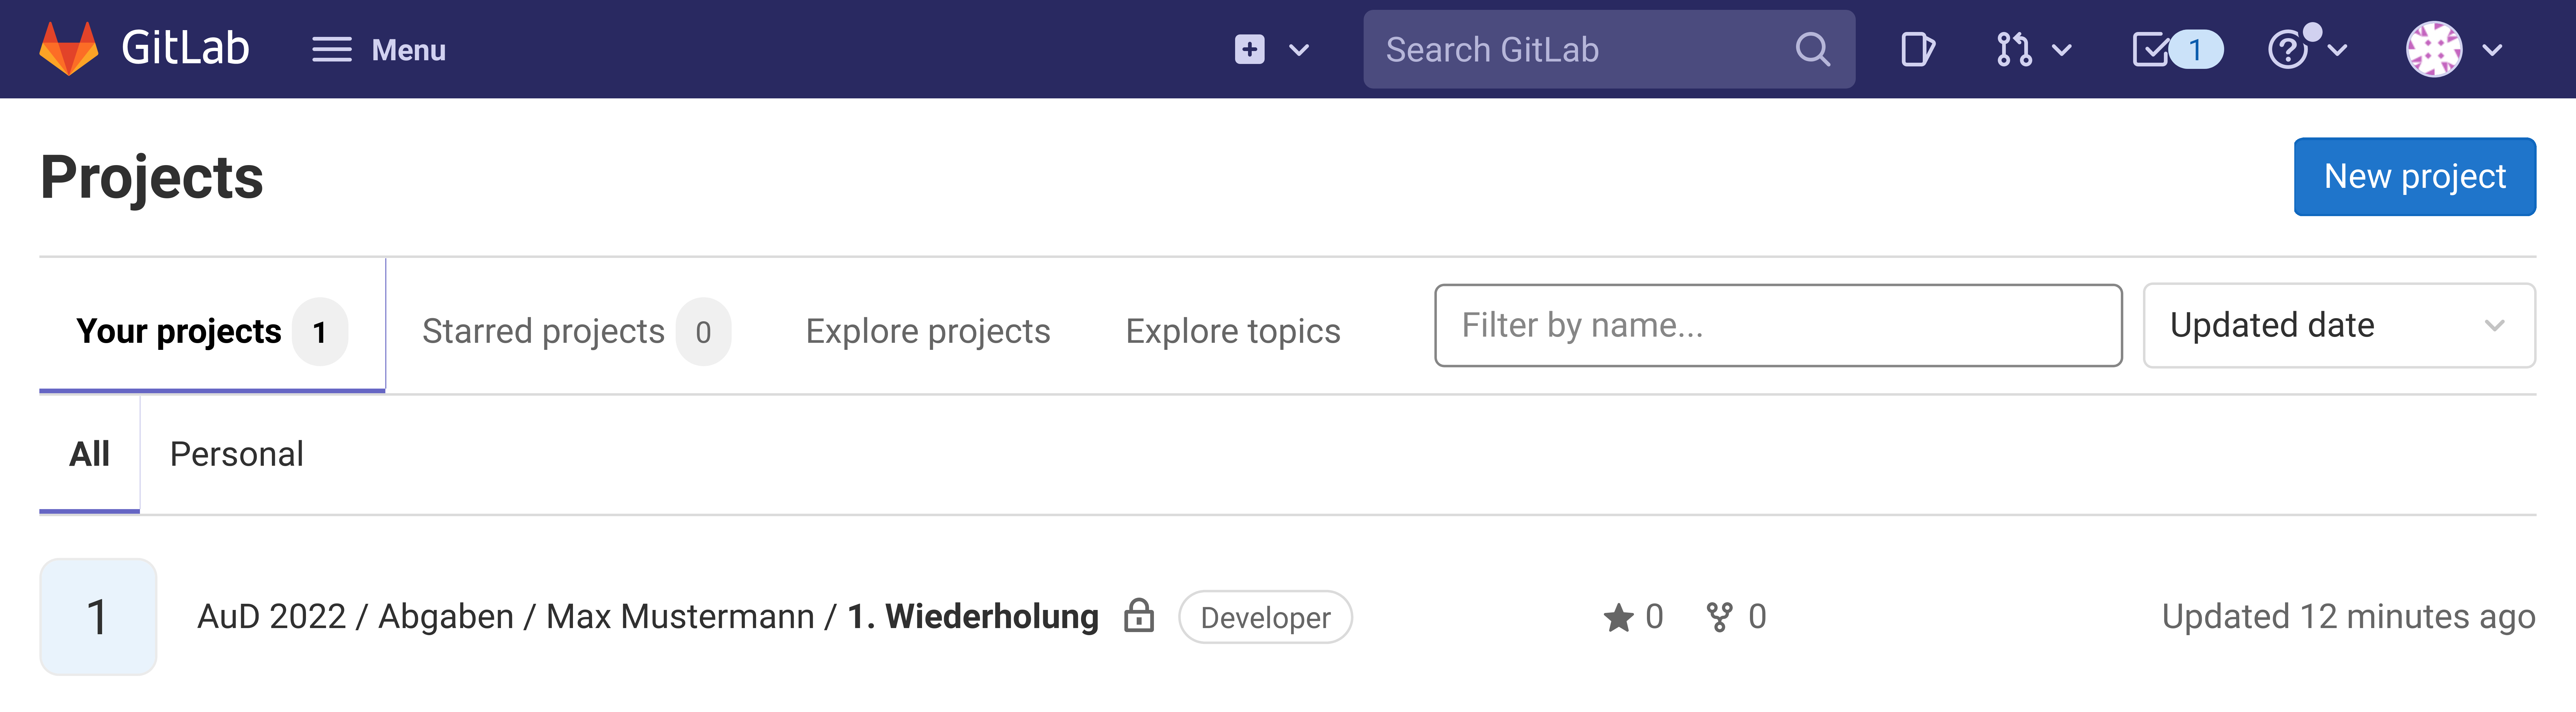
\includegraphics[width=0.9\textwidth]{img/de/screenshot-project-overview.png}
		\end{figure}
		
		\vfill

		Klicken Sie auf die Programmieraufgabe, die Sie bearbeiten wollen.
		
		\vfill

		\begin{tcolorbox}[title=\faLightbulbO\space Hinweis,colbacktitle=hintboxcolor,colframe=hintboxcolor]
			Falls Sie das GitLab vorher noch nie genutzt haben, werden Sie die 1. Programmieraufgabe nicht sofort nach dem Login in Ihrem Account sehen. Die Aufgabe sollte innerhalb einiger Stunden, max. 1 Werktag, erscheinen. Schauen Sie also später noch einmal nach.
		\end{tcolorbox}
		
		\vspace{6cm}
		
		\newpage
		
		\item Sie sehen nun eine Liste der Dateien, die zur Programmieraufgabe gehören, sowie die Aufgabenstellung:
		
		\vfill
		
		\begin{figure}[h!]
			\centering
			\includegraphics[width=0.9\textwidth]{img/de/screenshot-project.png}
		\end{figure}
		
		\vfill
		
		Zu jeder Programmieraufgabe gehören drei Dateien:
		
		\begin{itemize}
			\item \texttt{README.md} enthält die Aufgabenstellung.
			\item \texttt{StudentTestSuite.py} enthält Tests, mit denen Sie Ihre Lösung vor dem Abgeben überprüfen können.
			\item \texttt{solution.py} enthält das Grundgerüst der Lösung. Hier müssen Sie Ihre Implementierung einfügen.
		\end{itemize}
	
		\vfill
		
		\pagebreak
		
		\item Laden Sie die Dateien herunter, indem Sie auf das Download-Symbol \faDownload\space klicken:
		
		\vfill
		
		\begin{figure}[h!]
			\centering	
			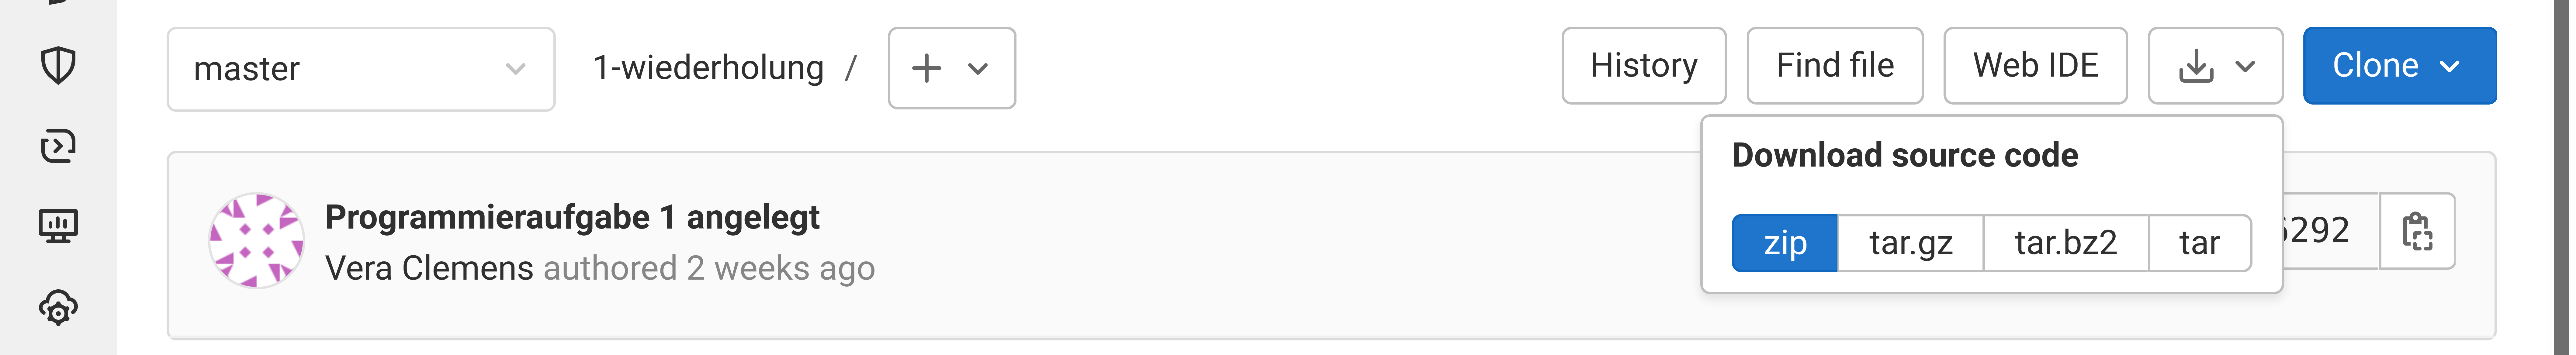
\includegraphics[width=0.9\textwidth]{img/de/screenshot-download.png}
		\end{figure}
		
%		\vfill
%		
%		\begin{tcolorbox}[title=\faLightbulbO\space Hinweis,colbacktitle=hintboxcolor,colframe=hintboxcolor]
%			Sie können auch das Git-Repository mit dem Button \enquote{Clone} herunterladen. Tun Sie das nur, falls Sie bereits Vorkenntnisse in Git haben und wissen, was Sie tun. Wir können dabei keine Unterstützung bieten.
%		\end{tcolorbox}
		
		\vfill
		
		\item Bearbeiten Sie nun die Programmieraufgabe, indem Sie Ihre Implementierung in \texttt{solution.py} entwickeln. Zwischendurch können Sie immer wieder überprüfen, ob Ihre Lösung für die Beispieleingaben richtig funktioniert, indem Sie die Tests ausführen. Öffnen Sie dazu ein Terminal in dem Verzeichnis, in dem Ihre Lösung und die Testdatei liegen, und führen Sie aus:
		
		\vfill
		
		\texttt{python3 -m unittest StudentTestSuite.py}
		
		\vfill
		
		Sie erhalten eine Ausgabe, die Ihnen sagt, ob Sie alle Testfälle bestehen oder nicht.
		
		\vfill
		
		\item Sobald Sie denken, dass Ihre Implementierung korrekt ist, können Sie sie auf GitLab abgeben.
		
		\vfill
		
		\begin{tcolorbox}[title=\faExclamationCircle\space Achtung,colbacktitle=red!75,colframe=red!75]
			\bfseries Sie haben für jede Programmieraufgabe nur 3 Abgabe-Versuche.
			
			Geben Sie keine Lösung ab, die nicht alle Testfälle in der Student-Test-Suite besteht!
			
			Achten Sie außerdem genau auf die allgemeinen Hinweise in der Aufgabenstellung (keine \texttt{import}- oder \texttt{input}-Anweisungen verwenden, kein Code außerhalb der gewünschten Funktionen,\ldots)!
		\end{tcolorbox}
	
		\vfill
	
		Klicken Sie dazu in der Dateiliste auf \texttt{solution.py}. 
		
		Klicken Sie dann auf \enquote{Replace}:
		
		\vfill
		
		
\includegraphics[width=0.9\textwidth]{img/screenshot-replace-button.png}
		
		\vspace{3cm}
		
		\pagebreak
		
		Fügen Sie Ihre Lösungsdatei ein und klicken dann auf \enquote{Replace file}:
		
		\vfill
		
		\begin{figure}[h!]
			\centering
			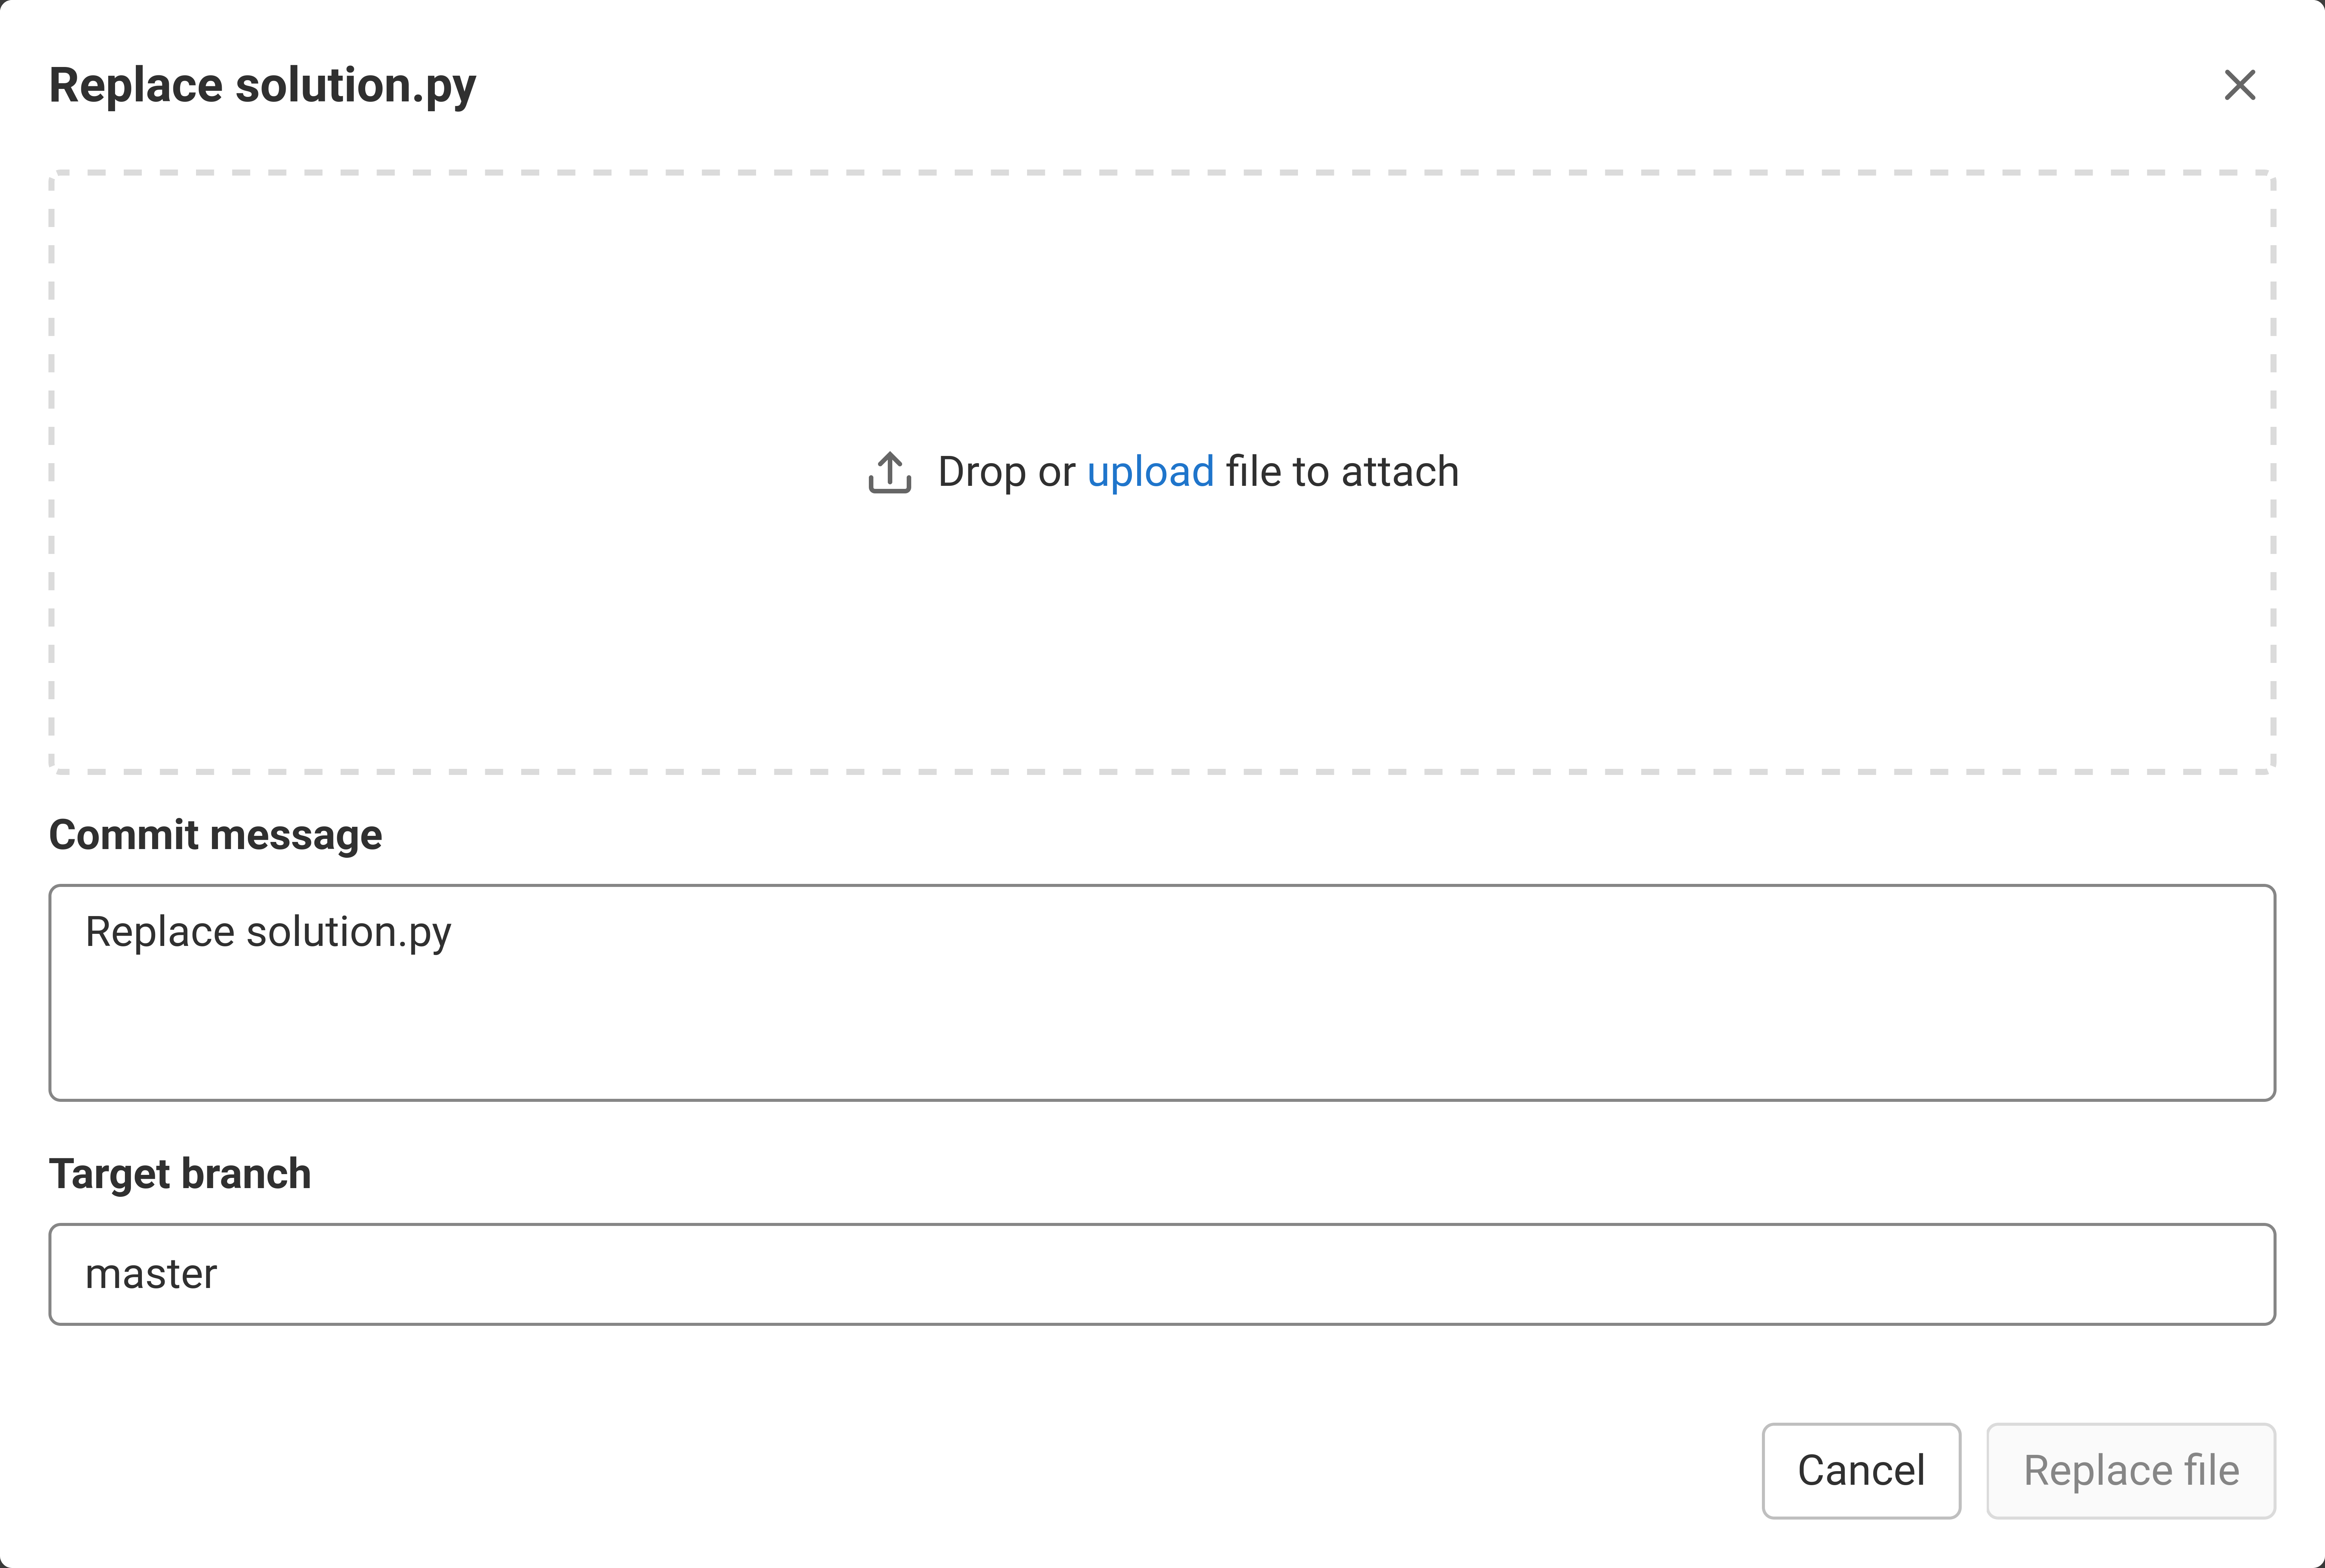
\includegraphics[width=0.75\textwidth]{img/screenshot-replace-dialog.png}
		\end{figure}
		
		\vfill
		
		Sie haben erfolgreich Ihre Lösung abgegeben!
		
		\vfill
		
		\item Jetzt wird Ihre Lösung automatisch überprüft. Wir nutzen dazu die Student-Test-Suite, die Ihnen zur Verfügung steht, aber zusätzlich auch noch weitere Tests. Wir überprüfen außerdem, ob Sie sich an die Hinweise in der Aufgabenstellung gehalten haben.
		
		Um die Ergebnisse der Überprüfung zu sehen, klicken Sie auf das bunte Icon neben Ihrer hochgeladenen Änderung:
		
		\vfill
		
		\begin{figure}[h!]
			\centering
			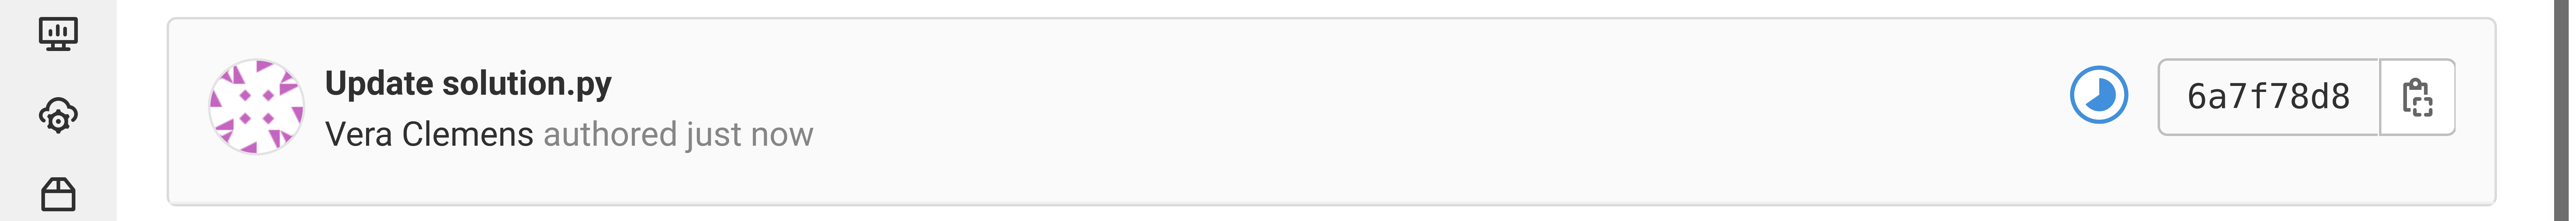
\includegraphics[width=0.9\textwidth]{img/screenshot-pipeline-icon.png}
		\end{figure}
		
		\vfill
		
		Solange die Überprüfung noch läuft, ist das Icon ein blauer Kreis, danach entweder ein grüner Haken oder ein rotes Kreuz.
		
		\vspace{3cm}
		
		\pagebreak
		
		\item Sie sehen nun die Ergebnisse der Überprüfung:
		
		\vfill
		
		\begin{figure}[h!]
			\centering
			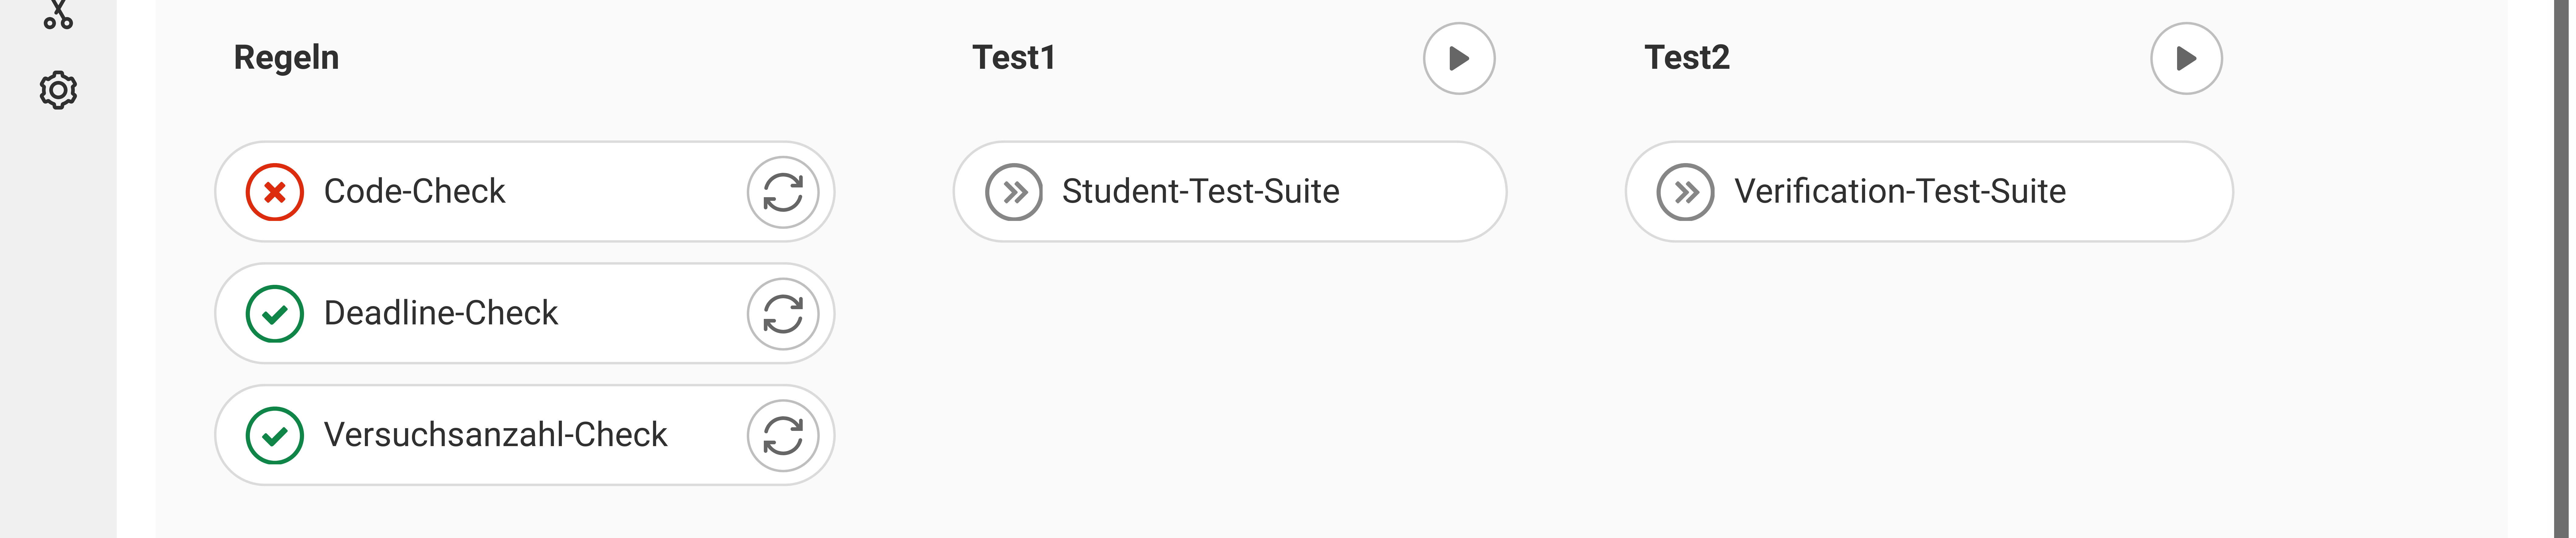
\includegraphics[width=0.9\textwidth]{img/de/screenshot-pipeline-results.png}
		\end{figure}
		
		\vfill
		
		Idealerweise sind alle Haken grün. Falls nicht (so wie hier), hat Ihre Lösung noch einen Fehler. Klicken Sie auf den jeweiligen Test, um einen Hinweis zu erhalten, wie Sie den Fehler lösen können, z.B.:
		
		\vfill
		
		\begin{figure}[h!]
			\centering		
			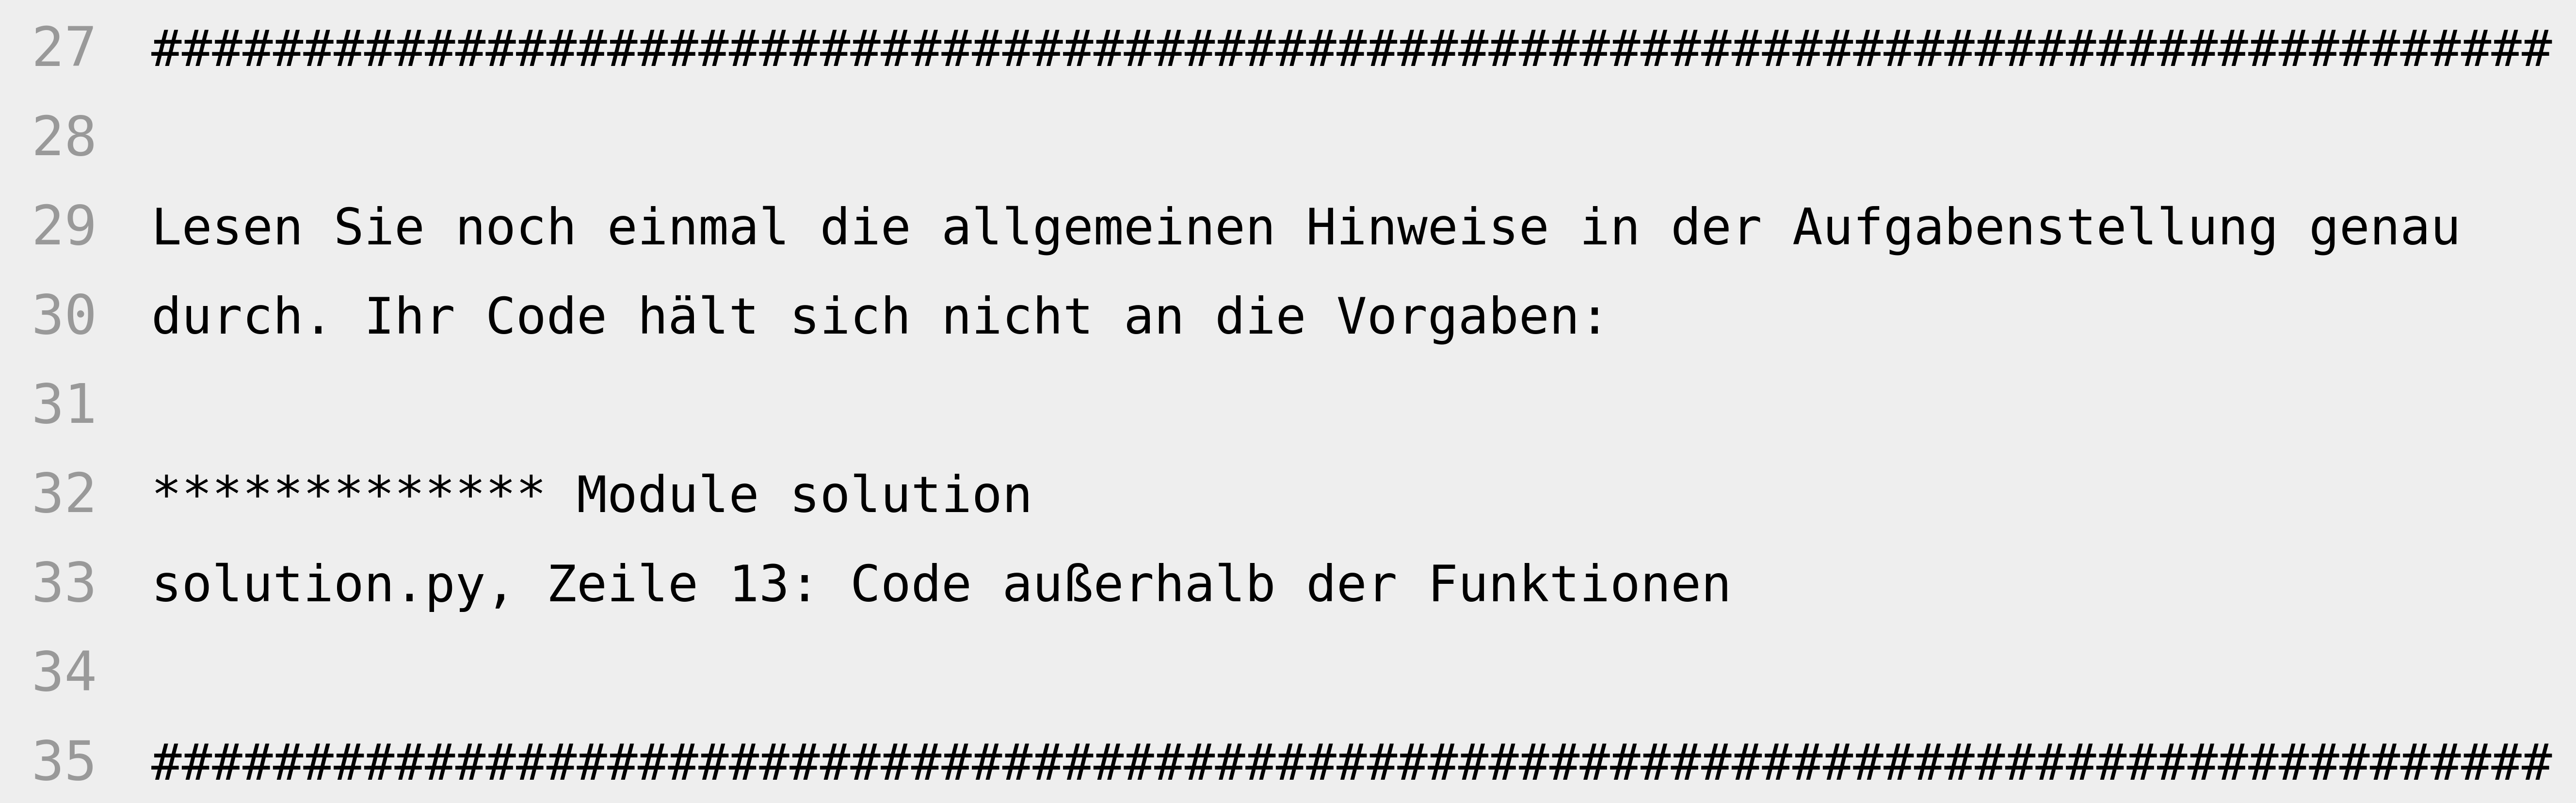
\includegraphics[width=0.75\textwidth]{img/de/screenshot-hint.png}
		\end{figure}
		
		\vfill
		
		\begin{tcolorbox}[title=\faLightbulbO\space Hinweis,colbacktitle=hintboxcolor,colframe=hintboxcolor]
			Wenn Sie auf \enquote{Versuchsanzahl-Check} klicken, wird Ihnen immer angezeigt, wie viele Abgabe-Versuche Sie noch haben.
			Unter \enquote{Deadline-Check} sehen Sie die verbleibende Zeit bis zur Deadline.
			
			\bfseries Alle Abgaben nach dem dritten Versuch oder nach der Deadline zählen nicht.
		\end{tcolorbox}
	
		\vfill
		
		\item Falls Sie Fragen zur Benutzung von GitLab oder zu den Programmieraufgaben haben, schreiben Sie einen Post im Fragen-Forum auf Moodle.
		
		\vfill
		
		{\Huge Viel Erfolg!}
		
		\vspace{3cm}
	\end{enumerate}
\end{document}